%-------------------------------------------------------------------------------
\section{Reusing Already Built Packages}
%-------------------------------------------------------------------------------
\label{sec:reuse}

While \spack{} is primarily a package manager installing software \emph{from sources}, the possibility to reuse  already built software more aggressively has been a critical request from the community since a few years (REFSURVEY).

Many packaging systems, including \spack{} itself before the adoption of \clingo, reuse builds via metadata hashes. This mechanism relies on the fact that, when an installation graph is concretized, each node in the DAG can be given a unique hash that identifies it, as shown in (FIGURE SLIDE 19). A user can then query for an exact hash match to reuse something that is either already installed or available in binary format in a buildcache. 

The issue with this way of proceeding is that users are \emph{effectively overconstraining} their request since specifying the hash is equivalent to specifying \emph{all the metadata} of the associated spec. This exposes users to need frequent changes in their configuration, since hashes are very sensitive to small changes, and prevents them from finding other satisfying specs that might be available.
% FIXME: expand on Nix, Guix, Conan etc. ?

\subsection{Optimizing for Software Reuse}
A more effective way to approach software reuse can be achieved by leveraging the ``Generalized Condition Handling'' logic shown in Section~\ref{subsec:generalizedcond}. 
First, all the metadata from installed packages need to be encoded into facts:
\begin{minted}[fontsize=\tiny, bgcolor=bg]{text}
installed_hash("zlib","7fatdw6gth5nlfdj4d463rdhrby6qvx3").
imposed_constraint("7fatdw6gth5nlfdj4d463rdhrby6qvx3","node","zlib").
imposed_constraint("7fatdw6gth5nlfdj4d463rdhrby6qvx3","version","zlib","1.2.11").
imposed_constraint("7fatdw6gth5nlfdj4d463rdhrby6qvx3","node_platform","zlib","linux").
imposed_constraint("7fatdw6gth5nlfdj4d463rdhrby6qvx3","node_os","zlib","ubuntu20.04").
imposed_constraint("7fatdw6gth5nlfdj4d463rdhrby6qvx3","node_target","zlib","icelake").
...
\end{minted}
The encoding is based on \texttt{imposed\_constraint} where the constraint ID is the hash associated with the installed package.
To minimize the number of build from sources, the solver is allowed to choose a hash for any package:
\begin{minted}[fontsize=\small, bgcolor=bg]{text}
{ hash(P, Hash) : installed_hash(P, Hash) } 1
 :- node(P).
\end{minted}
If a hash is chosen, then all the constraints associated with it must be imposed:
\begin{minted}[fontsize=\small, bgcolor=bg]{text}
impose(Hash) :- hash(P, Hash).
\end{minted}
Finally, the number of builds (i.e. of packages \emph{without} a hash) is minimized:
\begin{minted}[fontsize=\small, bgcolor=bg]{text}
build(P) :- not hash(P, _), node(P).
#minimize { 1@100,P : build(P) }.
\end{minted}

The trickiest point is how to choose at which priority the minimization of builds should be put in our multi-objective optimization criteria. The difficulty we face here stems from the different nature that an already built configuration has with respect to one that we still have to build. In the former case we can't change any aspect of the underlying graph, e.g. we can't choose a different version or a different set of variants to improve some optimization score, since the installed configuration is immutable. In the latter case instead, since we still have to build the software, we would like to choose the most recent version, use the preferred variants etc. 

Reasoning on this issue it becomes evident that having a single optimization criteria that account for both installed and non-installed software would always lead to unsatisfying behavior. For instance, if we optimized for minimizing builds at the highest priority and have no installed software to reuse, the solver would choose minimal DAGs even though that means using old versions or non-default values for variants. If a user asked to build e.g. \texttt{cmake} it would probably be unexpected to build one version without networking capabilities just because that permits to trim \texttt{openssl} and its dependencies from the graph!

The solution that \spack{} adopts is to split the optimization criteria into two identical ``buckets'', one for installed software and one for software that is yet to be built, and optimize for them at different priorities:
\begin{enumerate}
\item First, minimize the objectives for software to be built
\item Then, minimize the number of builds
\item Finally, minimize the objectives for already built software
\end{enumerate}
Minimizing the number of builds at a priority that is always higher than any other criteria for installed software, but always lower than any criteria for software to be built allow \spack{} to pick the best version available of what is installed without affecting in any way the choice criteria for the software that will be built. 

To conclude this section it is worth to show an example of how effective this approch is to reuse software. Figure~\ref{fig:noreuse} shows a concretization relying on purely hash-based software reuse. We can see that in this specific case no match was found and 20 installations need to be performed from sources. In Figure~\ref{fig:reuse} we show instead the same concretization happening with the reuse logic turned on. In this case 16 installed packages are actually acceptable to be reused and only 4 need to be built. Also, due to the priority chosen for minimizing the number of builds, it is actually acceptable to reuse \texttt{cmake} at version 3.21.1 even though the preferred version if it was to be built is 3.21.4.

\begin{figure}[h]
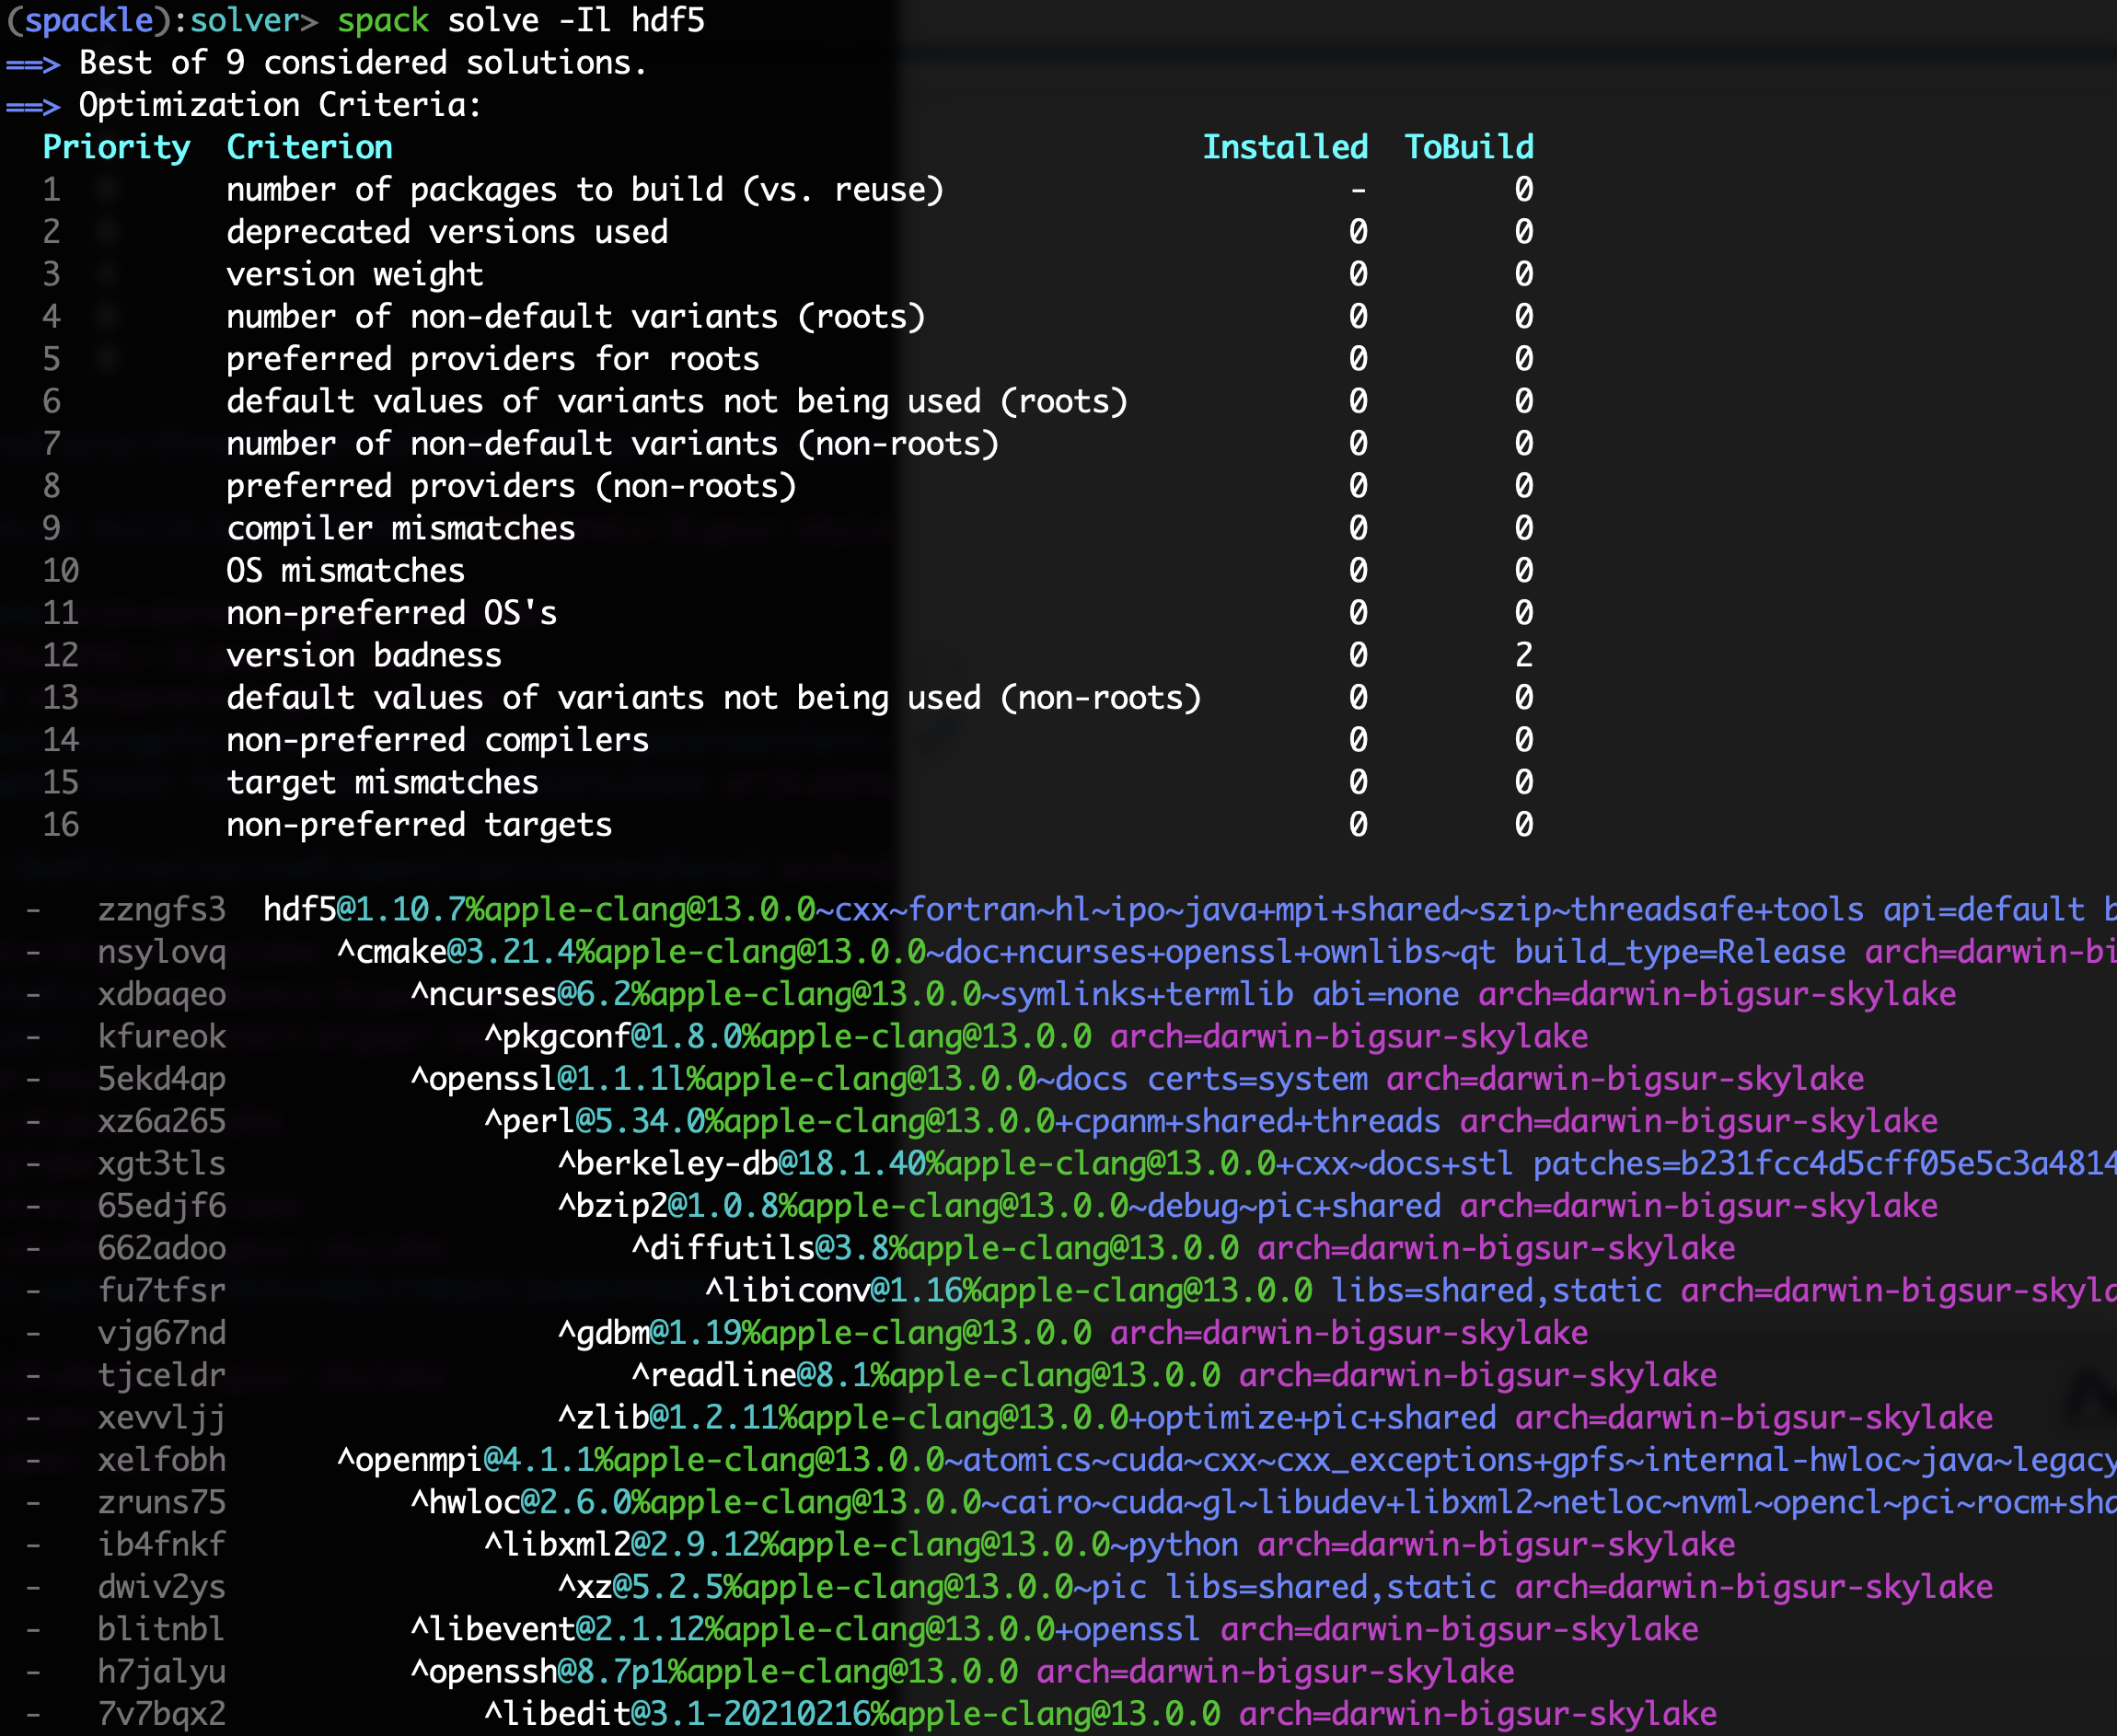
\includegraphics[width=\columnwidth]{figures/no-reuse.png}
\caption{Concretization of \texttt{hdf5} with pure hash-based reuse: all misses}
%\caption{The solver is asked to concretize \texttt{hdf5}. Without options, reusing software is purely hash-based and in this case it gives all misses.}
\label{fig:noreuse}
\end{figure}
\begin{figure}[h]
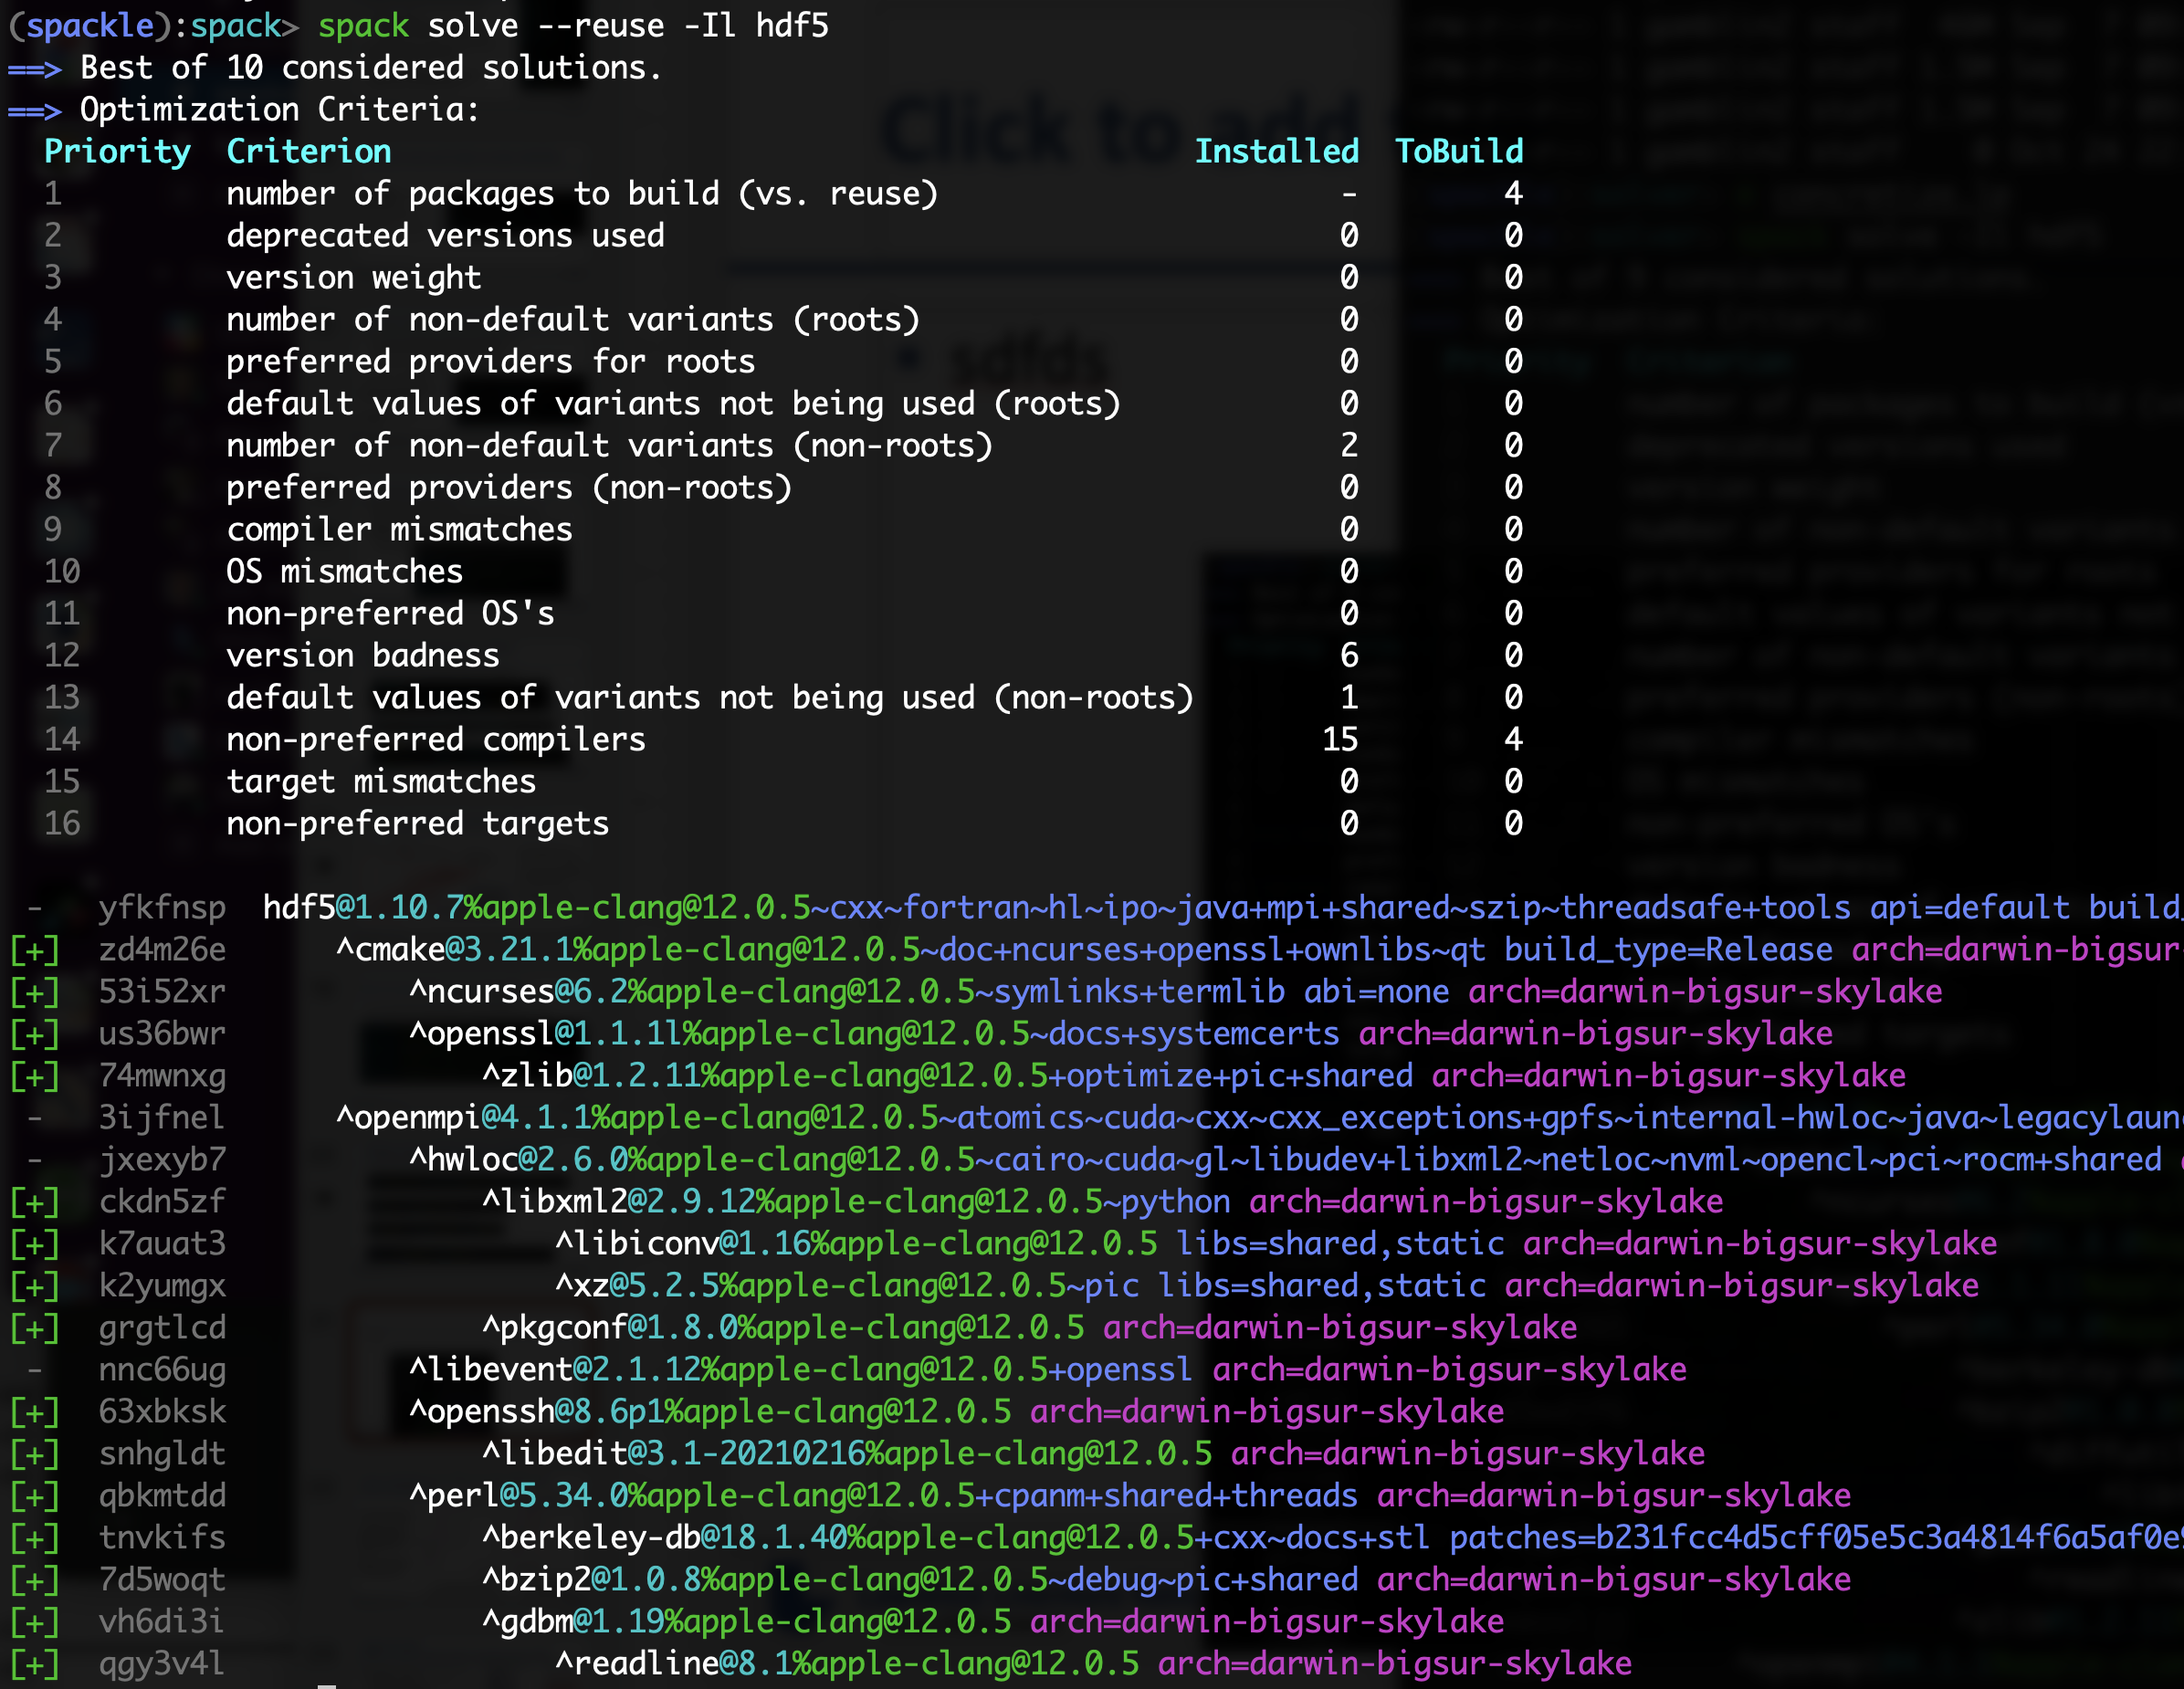
\includegraphics[width=\columnwidth]{figures/reuse.png}
\caption{Concretization of \texttt{hdf5} with reuse from \clingo: 16 packages were actually acceptable}
%\caption{The solver is asked to concretize \texttt{hdf5} trying to reuse installed software as much as possible. We see that 16 installed packages are actually acceptable to be reused. Another notable take is that, due to the priority chosen for minimizing the number of builds it is actually acceptable to \emph{reuse} \texttt{cmake} at version 3.21.1 even though the preferred version if it was to be built is 3.21.4}
\label{fig:reuse}
\end{figure}


%- reuse of half the generalized condition
%- Reusing built dependencies
%- architecting optimization criteria for builds vs. reuse